\section{Implementation}
The implementations created as part of this bachelor thesis aimed to make use of
the LLVM compiler infrastructure. LLVM is a collection of modular and reusable
compiler and tool chain technologies, most notably for this project is the clang
compiler. Furthermore, QEMU will be used extensively while testing the
implementations.

\subsection{Dependencies}
\subsubsection*{QEMU}
\begin{lstlisting}[caption=Installing QEMU, label=lst:qemu_install, float]
git clone git clone https://github.com/qemu/qemu  # Clone the QEMU repo
cd qemu
./configure --target-list=riscv32-softmmu  # Configure the 32-bit RISC-V target
make -j $(nproc)  # build the project with all num cores jobs
sudo make install
\end{lstlisting}
\begin{lstlisting}[caption=Installing LLVM compiler infastructure with RISC-V
32-bit as native target., label=lst:llvm_install, float]
# Dependencies
sudo apt-get -y install \
  binutils build-essential libtool texinfo \
  gzip zip unzip patchutils curl git \
  make cmake ninja-build automake bison flex gperf \
  grep sed gawk python bc \
  zlib1g-dev libexpat1-dev libmpc-dev \
  libglib2.0-dev libfdt-dev libpixman-1-dev

git clone https://github.com/riscv-collab/riscv-gnu-toolchain
cd riscv-gnu-toolchain  # change directory
./configure --prefix=/opt/riscv --with-arch=rv32gc -disable-linux --enable-llvm
sudo make -j$(nproc)
cd ..
popd
\end{lstlisting}
Following the instructions by RISC-V's getting started guide
we can build the QEMU RISC-V system emulators by running the code
provided in Listing~\ref{lst:qemu_install}\cite{RISC-V_GS}.

\subsubsection*{LLVM and RISC-V-gnu-toolchain}
Although the LLVM clang compiler comes with an available cross-compiler, I found
that it often caused issues with missing header files compatible with my
implementation. Furthermore, the lldb debugger was unable to provide a working
debugger for the multicore remote debugging on QEMU. These are issues, which
might only be affecting me, as information revolving the issues were scarce. As
such, the following steps of building llvm and the RISC-V 32-bit gdb might be
obsolete, but are left here as a known working toolchain. Running the code in
Listing~\ref{lst:llvm_install} installs a RISC-V compatible clang compiler and
gdb debugger in the /opt/riscv/ directory. For the use outside this folder, make
sure to add it to PATH.

\subsubsection*{libucontext}
Libucontext is an open sourced library which provides the ucontext.h C api. Most
notably for the project of this thesis, it is able to deploy on bare metal
RISC-V 32 bit with newlib. Building the library from scratch lead to some issues
on my end, and as such the necessary files were copied and linked together with
my implementation upon building. With this, I am able to use getcontext,
makecontext and setcontext, which allows me to do the necessary context
switching described within Section~\ref{sec:Design}.


\subsection{Creating a linker script}
The linker script is used to tell the linker which parts of the file to include
in the final output file, as well as where each section is stored in memory. As
we are working on an embedded system, we have to stray from the default and
create our own linker script. The clang uses the LLVM lld linker, which is
compatible with the general linker scripts implementations of the GNU ld linker
\cite{llvm-org-linker}. Thus, we can make use of the GNU ld manual for modifying
the linker script in freeRTOS for our bare metal application instead of writing
the entire thing from scratch \cite{GNU-linker}.

\begin{lstlisting}[caption=Memory area defined in linker script]
OUTPUT_ARCH('riscv')
ENTRY(_start)

MEMORY
{
/* Fake ROM area */
rom (rxa) : ORIGIN = 0x80000000, LENGTH = 1M
ram (wxa) : ORIGIN = 0x80100000, LENGTH = 127M
}
\end{lstlisting}
First, we must specify that we want the RISC-V architecture and designate the
entry point of the program at a function named '\_start,' which we will define
later. Second, we define the MEMORY area to consist of both a writable memory
region and a read-only memory region. We name these regions 'ram' and 'rom,'
respectively. With that, we move on to define the SECTIONS element of the linker
script.

\begin{lstlisting}[caption=Linker scripts SECTIONS.]
SECTIONS {
  .text : ALIGN(CONSTANT(MAXPAGESIZE))
  {
    *(.text .text.*)
  } > rom

  .rodata : ALIGN(CONSTANT(MAXPAGESIZE))
  {
    *(.rdata)
    *(.rodata .rodata.*)
  } > rom

  .data : ALIGN(CONSTANT(MAXPAGESIZE))
  {
    *(.data .data.*)
    /*RISCV convention to have __global_pointer aligned to 8 bytes*/
    . = ALIGN(8);
    PROVIDE( __global_pointer$ = . + 0x800 );
  } > ram

  .bss : ALIGN(CONSTANT(MAXPAGESIZE))
  {
    *(.bss .bss.*)
  } > ram

  /* It is standard to have
  the stack aligned to 16 bytes*/
  . = ALIGN(16);
  _end = .;

  .stack : ALIGN(CONSTANT(MAXPAGESIZE))
  {
    . = ALIGN(8);
    PROVIDE(_stack_start = .);
    PROVIDE(_stack_top = ORIGIN(ram) + LENGTH(ram));
  } > ram
}
\end{lstlisting}
The text, rodata, data and bss sections follow the same general procedure. We
align the section to the maximum size of a page, and match all the data which we
care about for the given sections. By specifying the > rom, we tell the linker
to save the given section in the rom section and the same is true for the > ram.
From the Figure~\ref{fig:mem_layout}, we can see the ram and rom correspond to
the ROM and RAM section of the figure.\footnote{rom stands for read-only memory,
and ram stands for random-access memory. Generally it is not necessarily needed
to split the two up as done here, but it is a good practice to separate what can
change and what cannot change in memory.}

In the data section, we also provide a global pointer, which is used to access
global variables within our later code implementation. The global pointer is
used together with an offset to save global variables. As such we allow for
0x800=2048 bytes of global variables. With the implementation being quite
reliant on global variables, it might need to be increased for lists of large
sizes.

The last section is the .stack section. We align the starting of the
\_stack\_start with 8 bytes. Generally not necessary in this instance, but still
a good custom. This is the point from where each thread stack will be allocated.
Next, we specify that the \_stack\_top will reside at the end of the ram
section, such that we can allocate a stack for each core with an offset.

\subsection{Getting into the main function}\label{sec:get_main}
In the linker script we specified the entry point of our program as \_start.
Next up is implementing said entry point in assembly. Within a new assembly file
we add the following.
\begin{lstlisting}[numbers=left, escapechar=|, caption=Assembly code for getting
to main function.]
.extern main |\label{line:header_start}|
.extern secondary_main
.globl _start
.type _start,@function
#include "../include/defines.h" |\label{line:header_end}|

_start: |\label{line:_start}|
  .cfi_startproc
  .cfi_undefined ra
  .option push
  .option norelax
  la gp, __global_pointer$
  .option pop |\label{line:pop}|
  // load _stack_top into the sp register
  la sp, _stack_top | \label{line:stack_top}|
  csrr a0, mhartid
  bnez a0, 2f | \label{line:break_zero}|
  1:
    // argc, argv is 0 and jump to main
    li  a0, 0
    li  a1, 0
    jal main | \label{line:jump_main} |
  1:
    // loop
    j 1b
  2:
    la t1, STACK_SIZE | \label{line:STACK_SIZE} |
    li t0, 0
  1:
    andi sp, sp, -16 | \label{line:align_stack} |
    beq a0, t0, 1f
    sub sp, sp, t1 | \label{line:sub_stack} |
    addi t0, t0, 1
    j 1b |\label{line:j_1b}|
  1: |\label{line:jump_secondary}|
    // argc, argv is 0 and jump to main
    li  a0, 0
    li  a1, 0
    jal secondary_main
  1:
    // loop
    j 1b
    .cfi_endproc  // We should never really reach this
\end{lstlisting}
Lines \ref{line:header_start}-\ref{line:header_end} provide the setup for the
assembly file. We specify that a main and secondary\_main label will be defined
outside of the file, that \_start is a global label and that \_start is a
function type. At last, we include the defines.h file, which includes
definitions of the STACK\_SIZE.

On lines \ref{line:_start}-\ref{line:pop} we give call frame information (cfi)
for there being no return address and that the process starts here. Then when
initializing the global pointer, we must specify options push, norelax, and pop
as described in GNU binutils. \cite{GNU_bin} After linker relaxation, this would
produce the expected code:
\begin{lstlisting}
auipc gp, %pcrel_hi(__global_pointer$)
addi gp, gp, %pcrel_lo(__global_pointer$)
\end{lstlisting}

On lines \ref{line:stack_top}-\ref{line:break_zero}, we load the value of
\_stack\_top, which the linker provides through the linker script defined
previously, and save it into the stack pointer(sp) register. We read the current
machine hart identifier(mhartid), which contains a unique identifier for each
core on the processor. This is what allows for differentiation between the
different cores. Line \ref{line:break_zero} moves execution to line
\ref{line:STACK_SIZE} if the machine hart identifier is not 0. As such, only
mhartid 0 will be allowed to continue execution to line \ref{line:jump_main},
where it jumps to the main function.

All other cores continue execution at line \ref{line:STACK_SIZE}, where they
load the value STACK\_SIZE defined in defines.h into the temporary register t1. We also load immediately(li) the value
1 into the temporary register r1. Line \ref{line:align_stack} aligns the current
value in the stack pointer to -16. Afterwards, we compare the value in
register a0, which holds the value of the mhartid, to the value in t0. If they
are equal, we jump to line \ref{line:jump_secondary}, which makes us jump to
the externally defined secondary\_main function. Otherwise, we continue on
line \ref{line:sub_stack}, where we subtract the register t1 (STACK\_SIZE)
from the value stored in the sp register. We increment the value in t0 by one,
and jump back to line \ref{line:align_stack}. With this loop, we are setting
up a stack of size STACK\_SIZE for all the different cores defined, such that
we get the desired memory layout shown at the top of
Figure~\ref{fig:mem_layout}.

\subsection{Initializing the thread jobs}\label{sec:init_threads}
\begin{algorithm}
  \begin{algorithmic}[1]
    \Require threads[] \# Empty thread array
    \Procedure {Initialize\_Threads}{$A$}
    \State $depth \leftarrow MostSignificantBit(NUM\_CORES)$
    \State $idx \leftarrow 0$
    \For{$i=0, i < depth$}
    \If{$i == 0$} \label{alg:early_escape}
    \State \# Top level thread
    \State $ct \leftarrow threads[idx]$
    \State mid \leftarrow Length(A)/2
    \State $thread\_create(ct, parallel\_merge)$
    \State $ct.l = 0$
    \State $ct.mid = mid$
    \State $ct.r = Length(A)$
    \State idx++
    \State \textbf{continue}
    \EndIf
    \State $k \leftarrow 2^k$
    \For{$j= 0, j < k$}
    \State $parent\_thread \leftarrow threads[(idx - 1)/2]$
    \State $ct \leftarrow thread[idx]$
    \If{$j \% 2 == 0$} \label{alg:left_right}
    \State $ct.l = parent\_thread.l$
    \State $ct.r = parent\_thread.mid$
    \Else
    \State $ct.l = parent\_thread.mid$
    \State $ct.r = parent\_thread.r$
    \EndIf
    \State $ct.mid = ct.l + (ct.r - ct.l)/2$ \label{alg:left_right_end}
    \If{$i == depth-1$} \label{alg:depth_check}
    \State \# Just regular merge sort
    \State thread\_create(ct, merge sort)
    \Else
    \State \# Merge given section
    \State thread\_create(ct, parallel\_merge)
    \EndIf
    \State idx++
    \EndFor
    \EndFor
  \EndProcedure
  \end{algorithmic}
  \caption{Initialization of the threads}\label{algo:threads}
\end{algorithm}
A pseudocode implementation for initializing the parallel merge sort algorithm is
provided in Algorithm~\ref{algo:threads}. Initially, it should be noted that it
is assumed NUM\_CORES is a multiple of 2. Next, as described in
Section~\ref{sec:singlevsmulti}, it is never in our interest to perform
unnecessary context switching when working on a single core. Consequently, we
can calculate the depth desired for our merge tree by employing the number of
cores. This may be achieved by taking $\log_2(NUM\_CORES)$ or, equivalently, by
examining the most significant bit of NUM\_CORES since it is a multiple of 2. At
line~\ref{alg:early_escape}, an early escape mechanism is implemented which
takes care of the single thread that will have no parent thread. If we are not
positioned at the very top level of the merge tree, we assign the variable 'k' as
the number of threads for the given level and partition the list to create
threads targeting a specific sub list. Lines \ref{alg:left_right} -
\ref{alg:left_right_end} address the task of determining which subsection of the
list each thread is responsible for. Finally, line~\ref{alg:depth_check} ensures
that we do not generate more active threads than what the available number of
cores can effectively handle. Upon completion of the algorithm, a threads array
will be produced containing $2 \cdot NUM\_CORES - 1$ different threads, each
assigned with a specific subsection of the list to either merge or perform
sequential merge sort on.

\subsection{Reducing synchronization}
\begin{figure}
  \begin{center}
    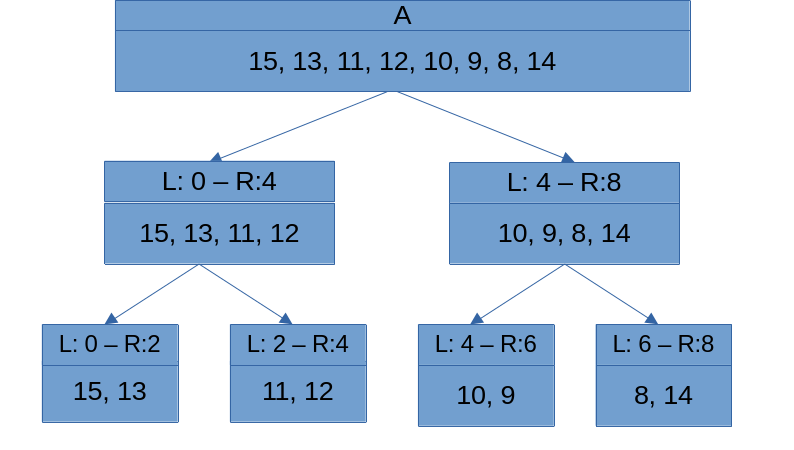
\includegraphics[width=0.85\textwidth]{figures/mergesort.png}
  \end{center}
  THREADS := [(A, 0, 8, MERGE), (A, 0, 4, MERGE), (A, 4, 8, MERGE), (A, 0, 2, MERGESORT),
  (A, 2, 4, MERGESORT), (A, 4, 6, MERGESORT), (A, 6, 8, MERGESORT)]
  \caption{Example of partitioning a random list using Algorithm~\ref{algo:threads}}\label{fig:mergesort}
\end{figure}

The idea behind initializing the threads array as described in
Section~\ref{sec:init_threads}, is  that we can reduce the need for
synchronization between threads, once the partitioning of the list is done. An
example can be seen in Figure~\ref{fig:mergesort} with the corresponding
finished THREADS array. This example would be on a system with 4 cores. As seen
in Section~\ref{sec:get_main} each core has a unique \textbf{id}, mhartid, from 0 to 3.
With this each core can index into the list with the number of jobs it has
already completed and the length of the array list, such that:
\begin{align}
  index &= LENGTH(A) - \text{NUM\_COMPLETED\_JOBS}\cdot id
\end{align}
With this, each thread is capable of retrieving a thread job without having to
consider the state of any other thread, as the job is preassigned during the
initialization. There are two caveats to this. Each merge must still wait on the
child thread (the direction of the arrow in Figure~\ref{fig:mergesort}) to
finish before starting a merge.



